\section{Using QGIS Core Plugins}\label{sec:core_plugins}\index{plugins!core}

% when the revision of a section has been finalized, 
% comment out the following line:
\updatedisclaimer

QGIS currently contains 11 core plugins that can be loaded using the Plugin 
Manager. Table \ref{tab:core_plugins} lists each of the core plugins along 
with a description of their purpose and the toolbar-icon.
Note the GRASS plugin is not included below because it installs its own 
toolbar (see section \ref{sec:grass} for a discussion of available features 
in the GRASS plugin).

% minipage is needed to appear the footnote under the table
% SH
\begin{minipage}{\textwidth}
\begin{table}[H]
\centering
\caption{QGIS Core Plugins}\label{tab:core_plugins}\medskip
\small
 \begin{tabular}{|l|l|p{4in}|}
\hline \textbf{Icon} & \textbf{Plugin} & \textbf{Description} \\
\hline

\includegraphics[width=0.7cm]{coordinate_capture}
 & Coordinate Capture \index{plugins!coordinate capture}& Capture mouse coordinate in different CRS\\
\hline 

\includegraphics[width=0.7cm]{copyright_label}
 & Copyright Label \index{plugins!copyright}& Display a copyright label on the map canvas\\
\hline 

\includegraphics[width=0.7cm]{delimited_text}
 & Delimited Text \index{plugins!delimited text}& Load a delimited text file 
containing x,y coordinates as a point layer \\
\hline 
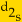
\includegraphics[width=0.7cm]{dxf2shp_converter}
 & DXF2Shape Converter \index{plugins!DXF2Shape}& Converts from DXF to SHP file format \\
\hline

\includegraphics[width=0.7cm]{georeferencer}
 & Georeferencer \index{plugin!georeferencer} & Georeferencing rasterlayers \\
\hline 

\includegraphics[width=0.7cm]{gps_importer}
 & GPS Tools \index{plugins!gps}& Load and display GPS data \\
\hline

\includegraphics[width=0.7cm]{grid_maker}
 & Graticule Creator \index{plugins!graticule}& Create a latitude/longitude grid and save as a shapefile\\
\hline

\includegraphics[width=0.7cm]{interpolation}
& Interpolation \index{plugins!Interpolation}& Interpolation on base of vertices of a vector layer\\
\hline

\includegraphics[width=0.7cm]{north_arrow}
& North Arrow \index{plugins!north arrow}& Add a north arrow to the map canvas\\
\hline

\includegraphics[width=0.7cm]{ogr_converter}
 & OGR Converter \index{plugins!OGR converter}& Translate vector between formats supported by OGR \\
\hline

\includegraphics[width=0.7cm]{icon_buffer}
 & PostgreSQL Geoprocessing \index{plugins!geoprocessing}& Buffer a PostGIS layer \\
\hline

\includegraphics[width=0.7cm]{quick_print}
 & Quick Print \index{plugins!quickprint}& Quickly print a map \\
\hline

\includegraphics[width=0.7cm]{scale_bar}
 & Scalebar \index{plugins!scalebar}& Add a scalebar to the map canvas\\
\hline

\includegraphics[width=0.7cm]{spiticon}
 & SPIT \index{plugins!spit}& Shapefile to PostGIS Import Tool - import shapefiles into PostgreSQL\\
\hline 

\includegraphics[width=0.7cm]{mIconAddWfsLayer}
 & WFS & Load and display WFS layer \\
\hline
\end{tabular}
\end{table}
\end{minipage}

\normalsize


\begin{Tip}\caption{\textsc{Plugins Settings Saved to Project}}\index{plugins
settings}
\qgistip{When you save a .qgs project, any changes you have made to NorthArrow, ScaleBar and Copyright plugins will be saved in the project and restored next time you load the project.
}
\end{Tip}


